\documentclass[compress]{beamer}
\mode<presentation>
\setbeamercovered{transparent}
\usetheme{Warsaw}
%\useoutertheme{smoothtree}
\usepackage{multirow}
\usepackage[english]{babel}
\usepackage[latin1]{inputenc}
\usepackage{times}
\usepackage[T1]{fontenc}
\usepackage{xmpmulti}
\usepackage{multicol}
\usepackage{colortbl}

%\setbeamersize{text margin left=.25 in,text margin right=.25 in}
\setbeamersize{text margin left=.15 in,text margin right=.15 in}
\usepackage[authoryear]{natbib}


\usepackage{epstopdf}
\usepackage{xcolor}
\usepackage{latexcolors}
%\usepackage[dvipsnames]{xcolor}
\definecolor{antiquebrass}{rgb}{0.8, 0.58, 0.46}
\definecolor{babyblueeyes}{rgb}{0.63, 0.79, 0.95}
\definecolor{babyblue}{rgb}{0.54, 0.81, 0.94}
\definecolor{bistre}{rgb}{0.24, 0.17, 0.12}
\definecolor{brightlavender}{rgb}{0.75, 0.58, 0.89}
\definecolor{bulgarianrose}{rgb}{0.28, 0.02, 0.03}
\definecolor{slateblue}{rgb}{0.56, 0.74, 0.56}
\definecolor{cordovan}{rgb}{0.54, 0.25, 0.27}
\definecolor{darkbyzantium}{rgb}{0.36, 0.22, 0.33}

\setbeamercolor{structure}{fg=bittersweet!70, bg= black!60}







\usepackage{tikz}
\usetikzlibrary{shadows,calc}
\usetikzlibrary{shadows.blur}
\usetikzlibrary{shapes.symbols}
\usepackage{hyperref}
\usepackage{booktabs}
\usepackage{colortbl}
\usepackage{multirow}
%%%%%%%%% shaddow image %%%%%
% some parameters for customization
\def\shadowshift{3pt,-3pt}
\def\shadowradius{6pt}
\colorlet{innercolor}{black!60}
\colorlet{outercolor}{gray!05}
% this draws a shadow under a rectangle node
\newcommand\drawshadow[1]{
\begin{pgfonlayer}{shadow}
    \shade[outercolor,inner color=innercolor,outer color=outercolor] ($(#1.south west)+(\shadowshift)+(\shadowradius/2,\shadowradius/2)$) circle (\shadowradius);
    \shade[outercolor,inner color=innercolor,outer color=outercolor] ($(#1.north west)+(\shadowshift)+(\shadowradius/2,-\shadowradius/2)$) circle (\shadowradius);
    \shade[outercolor,inner color=innercolor,outer color=outercolor] ($(#1.south east)+(\shadowshift)+(-\shadowradius/2,\shadowradius/2)$) circle (\shadowradius);
    \shade[outercolor,inner color=innercolor,outer color=outercolor] ($(#1.north east)+(\shadowshift)+(-\shadowradius/2,-\shadowradius/2)$) circle (\shadowradius);
    \shade[top color=innercolor,bottom color=outercolor] ($(#1.south west)+(\shadowshift)+(\shadowradius/2,-\shadowradius/2)$) rectangle ($(#1.south east)+(\shadowshift)+(-\shadowradius/2,\shadowradius/2)$);
    \shade[left color=innercolor,right color=outercolor] ($(#1.south east)+(\shadowshift)+(-\shadowradius/2,\shadowradius/2)$) rectangle ($(#1.north east)+(\shadowshift)+(\shadowradius/2,-\shadowradius/2)$);
    \shade[bottom color=innercolor,top color=outercolor] ($(#1.north west)+(\shadowshift)+(\shadowradius/2,-\shadowradius/2)$) rectangle ($(#1.north east)+(\shadowshift)+(-\shadowradius/2,\shadowradius/2)$);
    \shade[outercolor,right color=innercolor,left color=outercolor] ($(#1.south west)+(\shadowshift)+(-\shadowradius/2,\shadowradius/2)$) rectangle ($(#1.north west)+(\shadowshift)+(\shadowradius/2,-\shadowradius/2)$);
    \shade[outercolor,right color=innercolor,left color=innercolor] ($(#1.north west)+(-\shadowradius/12,\shadowradius/12)$) rectangle ($(#1.south east)+(\shadowradius/12,-\shadowradius/12)$);%Frame
    \filldraw ($(#1.south west)+(\shadowshift)+(\shadowradius/2,\shadowradius/2)$) rectangle ($(#1.north east)+(\shadowshift)-(\shadowradius/2,\shadowradius/2)$);
\end{pgfonlayer}
}
% create a shadow layer, so that we don't need to worry about overdrawing other things
\pgfdeclarelayer{shadow} 
\pgfsetlayers{shadow,main}
% Define image shadow command
\newcommand\shadowimage[2][]{%
\begin{tikzpicture}
\node[anchor=south west,inner sep=0] (image) at (0,0) {\includegraphics[#1]{#2}};
\drawshadow{image}
\end{tikzpicture}}
\usepackage{calligra}

\DeclareMathOperator*{\argmax}{Arg\,max}
\DeclareMathOperator*{\argmin}{Arg\,min}
\newcommand{\norm}[1]{\left\Vert #1 \right\Vert }
\newcommand{\bbetaHat}{ \widehat{\bbeta}}
\newcommand{\bbetaLSE}{ \widehat{\bbeta}_{_{\text{LSE}}}}
\newcommand{\bbetaMLE}{ \widehat{\bbeta}_{_{\text{MLE}}}}
\newcommand{\sqBullet}[1]{  {\tiny \tiny \tiny \qBoxCol{#1!60}{ }} }
%***************
%\newtheorem{thm}{Theorem}
%\documentclass[noinfoline]{imsart}
%\usepackage{amsmath,amstext,amssymb}
%%\usepackage[top=1.5in, bottom=1.5in, left=1.2in, right=1.2in]{geometry}
%% settings
%%\pubyear{2005}
%%\volume{0}
%%\issue{0}
%%\firstpage{1}
%%\lastpage{8}
%\arxiv{arXiv:0000.0000}

%\startlocaldefs
%\numberwithin{equation}{section}
%\theoremstyle{plain}
%\newtheorem{thm}{Theorem}
%\endlocaldefs
\usepackage{lipsum} 
\usepackage{amsmath}
\usepackage{amssymb}
\usepackage{amsbsy} 
\usepackage{amsthm}
\usepackage{mathrsfs}
\usepackage{eufrak}
\usepackage{mathrsfs}
\usepackage{color}
\usepackage{verbatim}
\usepackage{graphicx}
\usepackage{bm}
\usepackage{enumerate}
\usepackage{epstopdf} 
\usepackage{natbib}
\usepackage{undertilde}
%\RequirePackage[colorlinks,citecolor=blue,urlcolor=blue]{hyperref}
%\usepackage{subfig}
\usepackage[final]{pdfpages}

\usepackage{algorithm}  %@subhajit
\usepackage{algpseudocode} %@subhajit
\usepackage{algorithmicx}     %@subhajit
\usepackage{undertilde}


\newcommand{\sphere}{{\mathbb{S}}}
\newcommand{\R}{\mathbb{R}}
\newcommand{\LatentV}{V}
\newcommand{\NC}{m}
\newcommand{\Priorf}{f_{prior}}
\newcommand{\FWOne}[2]{{{}_{1}\Psi _{1}\left[{\begin{matrix}(\frac{#1}{2},\frac{1}{2})\\(1,0)\end{matrix}};#2\right]} 
}


\newcommand{\HyPriorMu}{\thetabf}
\newcommand{\HyPriorAlpha}{\alpha}
\newcommand{\HyPriorBeta}{\beta}
\newcommand{\HyPriorK}{\zeta}
\newcommand{\Indicator}[2]{\mathbb{I}_{_{#1}}({#2 })}
\newcommand{\xb}{\bm{x}}
\newcommand{\bx}{\MakeVec{\bm{x}}}
\newcommand{\bX}{\bm{X}}
\newcommand{\by}{\MakeVec{\bm{y}}}
\newcommand{\bZ}{\bm{Z}}
\newcommand{\bF}{\bm{F}}
\newcommand{\btheta}{\MakeVec{{\bm{\theta}}}}
\newcommand{\Bpi}{\MakeVec{\boldsymbol{\pi}}}
\newcommand{\thetabf}{\MakeVec{\boldsymbol{\theta}}}
\newcommand{\Thetabf}{\boldsymbol{\Theta}}
\newcommand{\taubf}{\MakeVec{\boldsymbol{\tau}}}
\newcommand{\Tr}{Tr}


\newcommand{\bM}{\bm{M}}
\newcommand{\bD}{\MakeVec{\bm{D}}}
\newcommand{\bV}{\MakeVec{\bm{V}}}
\newcommand{\loglikmix}{\mathcal{L}_{\bM,\bD,\bV}}
\newcommand{\hypdc}{{}_0F_1\left(\frac{n}{2},\frac{D_c^2}{4}\right)}


\usepackage{xstring}
\usepackage[normalem]{ulem}
\definecolor{ultramarine}{RGB}{38,29,163}
\newcommand\PalDel[1]{{\color{red} {\sout{#1}}}}
\newcommand\Pal[1]{{\color{ultramarine}{#1}}}
\newcommand\PalRp[2]{\PalDel{#1} \Pal{#2}}
\newcommand\PalCmnt[1]{{\color{ultramarine} {[[[***PAL:  #1 ***]]]}}}

\newcommand{\qedwhite}{\hfill \ensuremath{\Box}}
\newcommand{\SpaceD}{\mathcal{S}_p}
\newcommand{\SpaceM}{\widetilde{\mathcal{V}}_{n,p}}
\newcommand{\SpaceV}{\mathcal{V}_{p,p}}
\newcommand{\SpaceF}{\mathbb{R}^{n,p}}
\newcommand{\StiefelS}{\mathcal{V}_{n,p}}
\newcommand{\SpacePi}{\mathbb{S}_{\pi}}
\newcommand{\ML}{{\cal{ML}}}
\newcommand{\ProdSpace}{\boldsymbol{\Theta}}
\newcommand{\ThetaAndPi}{\Xi}
\newcommand{\ClassML}{\mathcal{C}_{\ML}}


\newcommand{\balpha}{\MakeVec{\bm{\alpha}}}
\newcommand{\bbeta}{\MakeVec{\bm{\beta}}}
\newcommand{\bEta}{\bm{\eta}}
\newcommand{\bd}{{\utilde{\bm{d}}}}
\newcommand{\BoEta}{{\utilde{\boldsymbol{\eta}}}}
%\newtheorem{theorem}{Theorem}[section]
%\newtheorem{theorem}{Theorem}
%\newtheorem{lemma}{Lemma}
%\newtheorem{result}{Result}
\newtheorem{defn}{Definition}
\newcommand{\pdv}[2][]{\frac{\partial#1}{\partial#2}}
\newcommand{\pdvtwo}[2][]{\frac{\partial^2#1}{{\partial#2}^2}}


%\newcommand{\mubf}{\boldsymbol{\mu}}
\newcommand{\mubf}{\MakeVec{\mu}}
\newcommand{\sumI}{ \sum_{i=1}^{n}}
\newcommand{\Ybar}{{\overline{Y}}}

\newcommand{\Expectation}[1]{\mathbb{E}{[#1]}}
\newcommand{\priorXzero}{\Psi}
\newcommand{\iMat}{\mathbf{I}_{p}}

% 
% \newtheorem{thm}{Theorem}[section]
% \newtheorem{cor}[thm]{Corollary}
% \newtheorem{lem}[thm]{Lemma}
%\newtheorem{proposition}{Proposition}

%\newtheorem{theorem}{Theorem}[chapter]%To link the theorem to each chapter uncomment the chapter option
%\newtheorem{lemma}{Lemma}%[theorem]% To link each lemma to a theorem uncomment the theorem option
%\newtheorem{corollary}{Corollary}%[theorem]% To link each corollary to a theorem uncomment the theorem option
% to link a corollary to a chapter change the theorem option to chapter
%\newtheorem{definition}{Definition}%[chapter] %the same is true for both definitions and assumptions
\newtheorem{assumption}{Assumption}%[chapter] %
%\newtheorem{proposition}{Proposition}[chapter]
%\newtheorem{fact}{Fact} %%% added by @subho
\newcommand{\StrongNBD}[2]{S_{#1}{#2}}
\newcommand{\bpi} {\boldsymbol{\pi}}
\newcommand{\bphi} {\boldsymbol{\phi}}
\newcommand{\bb}[1]{\boldsymbol{#1}}
% Definitions of handy macros can go here

\newcommand{\normtwo}[1]{{\left\lVert#1\right\rVert}_2}

\newcommand{\dataset}{{\cal D}}
\newcommand{\fracpartial}[2]{\frac{\partial #1}{\partial  #2}}
\newcommand{\Lesbegue}[1]{\mu_{\btheta_{#1},\bpi_{#1}}}
\newcommand{\fthetapi}[1]{f_{\btheta_{#1},\bpi_{#1}}}
% Heading arguments are {volume}{year}{pages}{submitted}{published}{author-full-names}
\newcommand{\doublehat}[1]{%
    \settoheight{\dhatheight}{\ensuremath{\widehat{#1}}}%
    \addtolength{\dhatheight}{-0.35ex}%
    \widehat{\vphantom{\rule{2pt}{\dhatheight}}%
    \smash{\hspace{-0.5mm}\widehat{#1}}}}

\newcommand{\hyp}{{}_0F_1\left(\frac{n}{2},\frac{D^2}{4}\right)}
\newcommand{\hypinline}{{}_0F_1\left({n}/{2},{D^2}/{4}\right)}

\newcommand{\partialhyp}[1]{\frac{\partial}{\partial\,{d_{#1}}}\,\left[\hyp\right]}

\newcommand{\fracProbZ}[1]{\frac{\langle Z_{ic} \rangle \, #1}{\sum_{i=1}^{N} \langle Z_{ic}\rangle  } }
\newcommand{\EmVar}[1]{\widetilde{#1}^{(c)}}

\newcommand{\IMDY}{{\it{CCPD}}}
\newcommand{\JMDY}{{\it{JCPD}}}

\newcommand{\DYlang}{\frac{\exp(\nu\,\bEta^T\bd)}{{\left[{}_0F_1\left(\frac{n}{2},\frac{D^2}{4}\right)\right]}^{\nu}}}

\newcommand{\logDYlang}{\nu\,\bEta^T\bd - \nu\,\log\left({}_0F_1\left(\frac{n}{2},\frac{D^2}{4}\right)\right)}

\newcommand{\lhyp}{\log\left({}_0F_1\left(\frac{n}{2},\frac{D^2}{4}\right)\right)}

%\jmlrheading{1}{2000}{1-48}{4/00}{10/00}{SS \& JH \& AB}

% Short headings should be running head and authors last names

%\ShortHeadings{BDP and cIBP}{SS \& JH \& AB}
%\firstpageno{1}

\newcommand{\diam}[1]{{{#1}^{\ast}}}

%%% coloring option %%%
\definecolor{auburn}{rgb}{0.53, 0.1, 0.5}
\newcommand{\sss}{\color{auburn}}  %%% for Subhajit
\newcommand{\sse}{\color{black}}
\newcommand{\attn}{\color{red}}
\newcommand{\rms}{\color{magenta}}  %%% for Riten
\newcommand{\rme}{\color{black}}
\newcommand{\MLDensity}{f_{\ML}}
\setlength{\parindent}{0cm}
\newcommand{\posterior}

\newcommand{\variableX}{\bd}
\newcommand{\funch}{\mathfrak{h}}
\newcommand{\IndVzero}[1]{\mathbb{I}({X\in \mathcal{V}^{#1}_0})}
\newcommand{\Rnp}{\mathbb{R}^{n \times p}}
\newcommand{\Rpp}{\mathbb{R}^{p \times p}}
\newcommand{\vecnorm}[1]{\lVert #1\rVert}

\newcommand{\etapsiD}{\eta_{\priorXzero}}
\newcommand{\BoEtapsiD}{\BoEta_{\priorXzero}}

\newcommand{\DMp}{\mathcal{D}^{p \times p}}
\newcommand{\Rplus}{\mathbb{R}_{+}}
\newcommand{\prodMeasure}{\Upsilon}

\newcommand{\m}{{\bf m_{\BoEta}}} 
\newcommand{\SetWithMode}{\mathcal{S}}
\newcommand{\SetWithModePrime}{\mathcal{S}}
\newcommand{\TargetComp}{\mathcal{S}^{\star}}

\newcommand{\ConstCondDen}{K_{\nu, \BoEta}} 

\newcommand{\hyparam}[2]{
    \IfEqCase{#1}{
        {M}{\xi^{#2}_c}
        {V}{\gamma^{#2}_c}%
        
    }
  }
\newcommand{\threepartdef}[6]
{
	\left\{
		\begin{array}{lll}
			#1 & \mbox{if } #2 \\
			#3 & \mbox{if } #4 \\
			#5 & \mbox{if } #6
		\end{array}
	\right.
}

\def\bv{\color{blue}}
\def\ev{\color{black}}
\newcommand{\bch}{\bv }
\newcommand{\ech}{\ev\normalsize}
%\newcommand{\MakeVec}[1]{{\utilde{\bf #1}}}
\newcommand \Measure[2][]{%
  \ifstrempty{#1}{
  \IfEqCase{#2}{
        {M}{\mu}%
        {D}{\mu_1}%
        {V}{\mu_2}
        {X}{\mu}
   }  
  }{
  \IfEqCase{#1}{
  {1}{
   \IfEqCase{#2}{
        {M}{d\mu(M)}%
        {D}{d\mu_1(\bd)}%
        {V}{d\mu_2(V)}
        {X}{d\mu(X)}
        {Y}{d\mu(Y)}
        {MDV} {d\mu(M)\; d\mu_1(\bd) \;d\mu_2(V) }
        }
   } 
   {2}{
   \IfEqCase{#2}{
         {M}{d\mu(M^{\ast})}%
        {D}{d\mu_1(\bd^{\ast})}%
        {V}{d\mu_2(V^{\ast})}
        {X}{d\mu(X^{\ast})}
        }
   }
   {3}{
   \IfEqCase{#2}{
         {M}{\mu(dM^{\star})}%
        {D}{\mu_2(d\bd^{\star})}%
        {V}{\mu_1(dV^{\star})}
        {X}{\mu(X^{\star})}
        }
   }   
   
   } 
  }%
}
  \newcommand{\VONF}{\text{VonMisesFisher}}
\newcommand{\MPGalpha}{\alpha}
\newcommand{\MPGnu}{\nu}
\newcommand{\MPG}{MPG }
\newcommand{\ybin}{y^{(\text{bin})}}


%\newcommand{\abs}[1]{\left \vert  #1  \right\vert  }
\usepackage{caption}
\usepackage{subcaption}

%%%%%%%%%%%%%%%%%%%%%%%%%%%
\newcommand{\IEHC}{\text{IEHC}}







\newcommand \Th[1]{%
  \IfEqCase{#1}{
        {1}{ 1^{\text{st}}}%
        {2}{2^{\text{nd}}}%
        {3}{3^{\text{rd}}}%
  }[{#1}^{\text{th}}]
}
  
  
   \newcommand{\augV}{\text{aux}}
  
  
  
  
  \newcommand{\CDE}{\text{PL}}
\newcommand{\CDEsigma}{\sigma}
\newcommand{\CDEepsilon}{\SVepsilon}
\newcommand{\CDEmu}{\mu}
 % \newcommand{\SVepsilon}{\varepsilon}
  \newcommand{\SVepsilon}{\delta}
 \newcommand{\abs}[1]{\left\lvert{#1}\right \rvert }
 
 
\newcommand{\CPDX }{\text{CPDX}}
\newcommand{\CPDXPar}{\vartheta}
\newcommand{\K}{\mathcal{K}}



\newcommand{\lossFunctionOne}[1]{ \left\{ \abs{ ( \abs{#1}-\SVepsilon)}  + ( \abs{#1}-\SVepsilon)\right\} }

\newcommand{\lossFunctionAlt}[1]{ \abs{  #1-\SVepsilon}  + \abs{ #1+\SVepsilon}-2\SVepsilon }

\newcommand{\lossFunctionAltOne}[1]{   \lossFunctionAlt{ \frac{\left(#1\right)}{\sigma}}}

\newcommand{\lossFunction}[1]{ \left\{ \abs{ \left( \frac{\abs{#1}}{\sigma}-\SVepsilon\right)}  + \left( \frac{\abs{#1}}{\sigma}-\SVepsilon\right)\right\} }
\newcommand{  \Likelihood}{\mathcal{L}}
%\newcommand{\Onebf}{\bf 1}
\newcommand{\Onebf}{{\bf \utilde{1}_{n}}}





\newcommand{\InvGamma}{\text{InvGamma}}
\newcommand{\PriorSigmaAlpha}{a}
\newcommand{\PriorSigmaBeta}{b}
\newcommand{\PriorBetaMean}{\mubf_{_{\bbeta}}}
\newcommand{\PriorBetaVar}{\Sigma_{_{\bbeta}}  }
\newcommand{\mvnormPdf}[4]{\frac{1}{ \left({2\pi}\right)^{\frac{#4}{2}} \sqrt{\vert{#3}\vert}}{\exp\left[ - \frac{1}{2}(#1- #2)^T {#3}^{-1} (#1- #2)\right]}      }
\newcommand{\InvGammaPdf}[3]{ \frac{(#1)^{-#2+1}}{\Gamma\left( #2\right) } \exp\left[ -\frac{{#3}}{{#1}} \right] }

 \newcommand{\byTilde}{\tilde{\by}}
 
 \newcommand{\TrfSigma}{\varsigma}
 \newcommand{ \Normal}{\text{Normal}}
 \newcommand{\GlobalPar}{\tau}
\newcommand{\LocalPar}{\psi}
\newcommand{\Not}[1]{{\overline{#1}}}
\newcommand{\st}{:}

\newcommand{\define}[2]{ \begin{definition}[#1]  #2  \end{definition}  }

\newcommand{\Exmpl}[2]{\qBrd[0.75in]{#1}{Example #2:}}
\newcommand{\Qn}{\HLTW{Question:} }


\newcommand{\pmf}{p}
\newcommand{\cdf}{F}
%\NewDocumentCommand{\support}{O{ }}{{\mathcal{S}}_{_{#1}}}
\NewDocumentCommand{\support}{O{ }}{{\mathbb{S}}_{_{#1}}}
%\newcommand{\SampleS}{\mathcal{S}}
\newcommand{\SampleS}{\mathscr{S}}
\usepackage{xcolor}
\usepackage{xparse}
\definecolor{lightGray}{gray}{0.95}
\definecolor{lightGrayOne}{gray}{0.9}
\definecolor{lightBlueOne}{RGB}{204, 255, 255}
\definecolor{lightBlueTwo}{RGB}{204, 238, 255}
\definecolor{lightBlueThree}{RGB}{204, 204, 255}
\definecolor{AltBlue}{RGB}{119,14,161}
\definecolor{Orchid}{RGB}{186,85,211}

\definecolor{BGBlue}{RGB}{220,221,252}
\definecolor{BGBlueOne}{RGB}{204,229,255}

\definecolor{DarkGreenOne}{RGB}{34,139,34}

\definecolor{BGGreen}{RGB}{240,243,245}
\definecolor{lightGreenOne}{RGB}{179, 255, 179}
\definecolor{lightGreenTwo}{RGB}{198, 255, 179}
\definecolor{lightGreenThree}{RGB}{243, 255, 230}
\definecolor{AltGreen}{RGB}{193, 240, 240}

\definecolor{BOGreen}{RGB}{180,0,0}
\definecolor{BGGreenOne}{RGB}{220,250,220}

\definecolor{lightBrownOne}{RGB}{255, 221, 204}
\definecolor{lightBrownTwo}{RGB}{255, 229, 204}
\definecolor{lightBrownThree}{RGB}{242, 217, 230}


\definecolor{HLTGreen}{RGB}{230,244,215}
\definecolor{ExcBrown}{RGB}{153,0,0}
\definecolor{ExcBGBrown}{RGB}{255,204,204}
\definecolor{BGYellowOne}{RGB}{255,235,208}
\definecolor{BGPink}{RGB}{255,215,240}

\newcommand{\MakeVec}[1]{{\utilde{\bf #1}}}

\NewDocumentCommand{\MCOption}{O{1.75in} m}{
\TextInBoxTwo[BGPink]{ #1 } {\TextInBoxTwo[white]{.1 in }{ \quad}\HLT{#2}}
}

 \NewDocumentCommand{\ThreeChoices}{O{Do not Know}O{Not confident}O{Confident}}{
\MCOption{#1} \MCOption{#2} \MCOption{#3}
}
 
\NewDocumentCommand{\OneBlock}{ O{HLTGreen} m m }{\colorbox{#1}{\begin{minipage}{#2} $ #3$ \end{minipage}}}

\NewDocumentCommand{\HLT}{ O{HLTGreen} m }{\colorbox{#1}{#2}}
%\NewDocumentCommand{\HLTEQ}{ O{HLTGreen} m }{\colorbox{#1}{$#2$}}
\NewDocumentCommand{\HLTEQ}{ O{white} m }{\colorbox{#1}{$#2$}}

%\newcommand{\HLT}[1]{\colorbox{HLTGreen}{#1}}
\newcommand{\DEHLT}[1]{\colorbox{lightGrayOne}{\color{white} #1}}

\newcommand{\TextInBoxOne}[2]{  {\fcolorbox{white}{lightGrayOne}{\begin{minipage}{#1}  #2 \end{minipage}}}}


\NewDocumentCommand{\TextInBoxTwo}{ O{lightGrayOne} m m } {{\fcolorbox{white}{#1}{\begin{minipage}{#2} { #3} \end{minipage}}}}


\newcommand{\TextInBox}[2]{  {\fcolorbox{BGGreen}{BGGreen}{\begin{minipage}{#1}  #2 \end{minipage}}}}
\newcommand{\TextInBoxCol}[2]{
\fcolorbox{BGBlue}{BGBlue}{%
\begin{minipage}{#1}
 {\color{AltBlue} #2}
\end{minipage}}%
}

\NewDocumentCommand{\TxtBnd}{ O{lightBrownOne} m m } {{\fcolorbox{white}{#1}{\begin{minipage}{#2} { #3} \end{minipage}}}}


\newcommand{\BandInTopBox}[2]{
\fcolorbox{AltBlue}{AltBlue}{%
\begin{minipage}{#1}{ {\color{white}  #2 \hspace{.1in}} }
\end{minipage}}%
}


\newcommand{\TextInBoxThm}[2]{
\fcolorbox{AltBlue}{lightGray}{%
\begin{minipage}{#1}
 {\color{black} #2}
\end{minipage}}%
}

\newcommand{\TextInBoxThmOne}[2]{
\fcolorbox{BGBlue}{BGBlueOne}{%
\begin{minipage}{#1}
 {\color{AltBlue} #2}
\end{minipage}}%
}

\newcommand{\TextInBoxLem}[2]{
\fcolorbox{BGBlue}{lightGray}{%
\begin{minipage}{#1}
 {\color{black} #2}
\end{minipage}}%
}



\newcommand{\TextInBoxLemOne}[2]{
\vspace{.02 in}
\noindent
\fcolorbox{BGBlue}{BGBlue}{%
\begin{minipage}{#1}
 {\color{AltBlue} #2}
\end{minipage}}%
}



\newcommand{\DefBox}[1]{
%\vspace{.1 in}
\noindent
\TextInBoxLem{4.5 in }{
\BandInTopBox{4.4 in }{}
\TextInBoxLemOne{4.4 in }{
#1
}}}





\newcommand{\DefBoxOne}[2]{
%\vspace{.1 in}
\noindent
\TextInBoxLem{4.5 in }{
\BandInTopBox{4.4 in }{#1}
\TextInBoxLemOne{4.4 in }{
#2
}}}


\newcommand{\ThmBox}[2]{
\noindent
\TextInBoxThm{4.4 in }{
\TextInBoxThmOne{4.4 in }{
#1}
#2}
}

\newcommand{\LemBox}[2]{
\noindent
\TextInBoxLem{4.5 in }{
\TextInBoxLemOne{4.4 in }{
#1}
#2}
}

\newcommand{\PropBox}[2]{
\vspace{.1 in}
\noindent
\TextInBoxLem{4.5 in }{
\TextInBoxLemOne{4.4 in }{
#1}
#2}
}




\newcommand{\TextInBoxExc}[2]{
\noindent
\fcolorbox{white}{BGGreenOne}{%
\begin{minipage}{#1}
 {\color{black} #2}
\end{minipage}}%
}


\newcommand{\TextInBoxExample}[2]{
\noindent
\fcolorbox{white}{BGPink}{%
\begin{minipage}{#1}
 {\color{black} #2}
\end{minipage}}%
}


\newcommand{\ExerciseBox}[1]{
\noindent
%\TextInBoxLem{6 in }{
\TextInBoxExc{6 in }{
#1}
%#2}
}


\newcommand{\ExampleBox}[1]{
\noindent
%\TextInBoxLem{6 in }{
\TextInBoxExample{6 in }{
#1}
%#2}
}

\NewDocumentCommand{\CommentBox}{ O{BGBlue}  m }{
\TextInBoxLem{5.5in }{
{\bf Comment:}\\
\TextInBoxLemOne{5.4 in }{
#2}}
}



\newcommand{\HLTY}[1]{\HLTEQ[yellow]{#1}}
\newcommand{\HLTW}[1]{\HLTEQ[white]{#1}}



\newcommand{\qBox}[1]{
  \begin{tikzpicture}
\node[draw=none,shade,
      top color=lightGrayOne,
      bottom color=lightGray,
      rounded corners=2pt,
      blur shadow={shadow blur steps=5}
    ] at (0,0) {    \noindent 
\fcolorbox{white}{BGBlue}{%
\begin{minipage}{4.55 in}
 {\color{black} {
 #1}}
\end{minipage}  }%
 };
 
    \end{tikzpicture}
}
 
 


 

\newcommand{\qBoxCol}[2]{
  \begin{tikzpicture}
\node[draw=none,shade,
      top color=lightGrayOne,
      bottom color=lightGray,
      rounded corners=2pt,
      blur shadow={shadow blur steps=5}
    ] at (0,0) {    \noindent
\fcolorbox{white}{#1}{%
%\begin{minipage}{4.55 in}
\begin{minipage}{4.55 in}
 {
 \color{black} {
 #2}}
\end{minipage}  }%
 };
 
    \end{tikzpicture}
}
  
  
  
  
  
  

\NewDocumentCommand{\qBrd}{O{4.55 in} m m}{
  \begin{tikzpicture}
\node[draw=none,shade,
      top color=#2,
      bottom color=#2,
      rounded corners=2pt,
      blur shadow={shadow blur steps=5}
    ] at (0,0) {    \begin{minipage}{#1}
 {
 \color{black} {
 #3}}
\end{minipage} 

 };
 
    \end{tikzpicture}
}
    
  
  
  
  
\NewDocumentCommand{\qbx}{O{4.55 in} m m}{
  \begin{tikzpicture}
\node[draw=none,shade,
      top color=lightGrayOne,
      bottom color=lightGray,
      rounded corners=2pt,
      blur shadow={shadow blur steps=5}
    ] at (0,0) {    \noindent
\fcolorbox{white}{#2}{%
%\begin{minipage}{4.55 in}
\begin{minipage}{#1}
 {
 \color{black} {
 #3}}
\end{minipage}  }%
 };
 
    \end{tikzpicture}
}
  
 
 
 \newcommand{\CurlyBox}[1]{
\begin{center}
  \begin{tikzpicture}
    \node[tape,draw=none,shade,
      top color=blue!40,
      bottom color=blue!5,
      rounded corners=1pt,
      blur shadow={shadow blur steps=5,shadow blur extra rounding=1.3pt}
    ] at (2,0){\sffamily\bfseries\large #1};
  \end{tikzpicture}
\end{center} 
 }


\newcommand{\CmntBnd}{\BandInTopBox{4.5in}{Comment:}}
\NewDocumentCommand{\TopBand}{O{Comment:} m}{ \BandInTopBox{4.5in}{#2}}

\newcommand{\DBX}[1]{
 	\HLTEQ[AltBlue]{
 				\HLTEQ[BGBlue]{  #1  }
 	}
 }



\NewDocumentCommand{\TransitionFrame}{O{slateblue}m}{
\begin{frame}{ }
\qBoxCol{#1!40}{\vspace{.8in}  \begin{center}\qBrd[2in]{#1!70}{ \begin{center} \vspace{.1in}
  #2 \\
 \vspace{.1in}
\end{center}}\end{center}
\vspace{.7in}
}

\end{frame}

}


\newcommand \rbind[1]{%
    \saveexpandmode\expandarg
    \StrSubstitute{\noexpand#1}{,}{&}[\fooo]%
    %\StrSubstitute{\fooo}{,}{&}[\fooo]%
    \StrSubstitute{\fooo}{;}{\noexpand\\}[\fooo]%
    \StrSubstitute{\fooo}{:}{\noexpand\\}[\fooo]%
    \restoreexpandmode
   \left[ \begin{matrix}\fooo\end{matrix}\right]
    }
    
    
    
   \newcommand \ColVec[1]{%
    \saveexpandmode\expandarg
    \StrSubstitute{\noexpand#1}{,}{\noexpand\\}[\fooo]%
    %\StrSubstitute{\fooo}{,}{&}[\fooo]%
    \StrSubstitute{\fooo}{;}{\noexpand\\}[\fooo]%
    \StrSubstitute{\fooo}{:}{\noexpand\\}[\fooo]%
    \restoreexpandmode
   \left[ \begin{matrix}\fooo\end{matrix}\right]
    }
     \newcommand \RowVec[1]{%
    \saveexpandmode\expandarg
    \StrSubstitute{\noexpand#1}{,}{&}[\fooo]%
    %\StrSubstitute{\fooo}{,}{&}[\fooo]%
    \StrSubstitute{\fooo}{;}{&}[\fooo]%
    \StrSubstitute{\fooo}{:}{&}[\fooo]%
    \restoreexpandmode
   \left[ \begin{matrix}\fooo\end{matrix}\right]
    }



  \newcommand \Row[1]{%
    \saveexpandmode\expandarg
    \StrSubstitute{\noexpand#1}{,}{&}[\fooo]%
    %\StrSubstitute{\fooo}{,}{&}[\fooo]%
    \StrSubstitute{\fooo}{;}{&}[\fooo]%
    \StrSubstitute{\fooo}{:}{&}[\fooo]%
    \restoreexpandmode
    \begin{matrix}\fooo\end{matrix}
    }
        
    
    
    
    \newcommand \Col[1]{%
    \saveexpandmode\expandarg
    \StrSubstitute{\noexpand#1}{,}{\noexpand\\}[\fooo]%
    %\StrSubstitute{\fooo}{,}{&}[\fooo]%
    \StrSubstitute{\fooo}{;}{\noexpand\\}[\fooo]%
    \StrSubstitute{\fooo}{:}{\noexpand\\}[\fooo]%
    \restoreexpandmode
    \begin{matrix}\fooo\end{matrix}
    }

%%%%%%%%%%%%%%%%%%%%% Experimental %%%%%%%%%%%%%%%%%


\ExplSyntaxOn
\DeclareExpandableDocumentCommand{\replicate}{O{}mm}
 {
  \int_compare:nT { #2 > 0 }
   {
    {#3}\prg_replicate:nn {#2 - 1} { #1#3 }
   }
 }
\ExplSyntaxOff


\ExplSyntaxOn
\DeclareExpandableDocumentCommand{\repdiag}{O{}mm}
 {
  \int_compare:nT { #2 > 0 }
   {
    {\prg_replicate:nn {#2}{#3#1}}{#3}
   }
 }
\ExplSyntaxOff


\newcommand \StrRowDiag[1]{%
    \saveexpandmode\expandarg
    \StrSubstitute{\noexpand#1}{,}{&}[\fooo]%
    %\StrSubstitute{\fooo}{,}{&}[\fooo]%
    \StrSubstitute{\fooo}{;}{&}[\fooo]%
    \StrSubstitute{\fooo}{:}{&}[\fooo]%
    \StrCount{\fooo}{&}[\countfooo]
    \restoreexpandmode
    \repdiag[0]{\countfooo+1}{{,}}
   %\left[ \begin{matrix}\fooo\end{matrix}\right]
    }


\newcommand \DiagStrOne[2]{%
    \saveexpandmode\expandarg
    \StrSubstitute{\noexpand#1}{,}{\noexpand#2}[\fooo]%
    \restoreexpandmode
   %\left[ \begin{matrix}\fooo\end{matrix}\right]
   \fooo
    }
    
    \newcommand \DiagStr[1]{%
    \DiagStrOne{#1}{{\StrRowDiag{#1}}}
    }


%$\rbind{\replicate[,]{10}{\Col{\replicate[;]{7}{0}}}}$

%$\Col{1,2,3}$
%$\ColVec{\replicate[;]{5}{B}}$
%$ \StrRowDiag{1,2} $

%$\DiagStr{1,2,3}$

%\repdiag[-]{3}{A}
\ExplSyntaxOn
\NewDocumentCommand{\Split}{ m m o }
 {
  \tarass_split:nn { #1 } { #2 }
  \IfNoValueTF { #3 } { \tl_use:N } { \tl_set_eq:NN #3 } \l_tarass_string_tl
 }

\tl_new:N \l_tarass_string_tl

\cs_new_protected:Npn \tarass_split:nn #1 #2
 {
  \tl_set:Nn \l_tarass_string_tl { #2 }
  % we need to start from the end, so we reverse the string
  \tl_reverse:N \l_tarass_string_tl
  % add a comma after any group of #1 tokens
  \regex_replace_all:nnN { (.{#1}) } { \1\, } \l_tarass_string_tl
  % if the length of the string is a multiple of #1 a trailing comma is added
  % so we remove it
  \regex_replace_once:nnN { \,\Z } { } \l_tarass_string_tl
  % reverse back
  \tl_reverse:N \l_tarass_string_tl
 }
\ExplSyntaxOff

%%%%%%%%%%%%%%%%%%%%%%%%%%%%%%%%

\newcommand{\ShowRowMatrix}[3]{ \left[ {\begin{array}{ccc}
  \line(1,0){22} &{#1} &  \line(1,0){22} \\
     & \vdots& \\
  \line(1,0){22}  &{#2}& \line(1,0){22} \\
   &  \vdots & \\
    \line(1,0){22} &{#3}& \line(1,0){22}  \\
    \end{array}
   } \right]}
 


\newcommand{\ShowColMatrix}[3]{ \left[ {\begin{array}{ccccc}
  \line(0,1){25} & &\line(0,1){25} &  &  \line(0,1){25} \\
  {#1}  & \ldots & {#2} &\ldots   &{#3} \\
 \line(0,1){25} &  & \line(0,1){25}  &  &  \line(0,1){25} \\
    \end{array}
   } \right]}
   
   
   
   
\newcommand{\ShowRowVector}[1]{ \left[ {\begin{array}{ccc}
  \line(1,0){25} &{#1} &  \line(1,0){25} 
    \end{array}
   } \right]}   
   
   
\newcommand{\ShowColVector}[1]{ \left[ {\begin{array}{c}
  \line(0,1){25} \\    {#1} \\   \line(0,1){25}     \end{array}  } \right]}
  
\newcommand{\ColVector}[3]{ \left[ {\begin{array}{c}
  {#1}\\ \vdots \\    {#2}\\ \vdots\\{#3}  \end{array}  } \right]}
  
  
  
  
  
\newcommand{\EqSetThree}[3]{ \left\{ {\begin{array}{c}
  {#1}\\ \vdots \\    {#2}\\ \vdots\\{#3}  \end{array}  } \right.}  
  



\newcommand{\MatrixTypeA}[3]{ \left[ {\begin{array}{ccc}
 {#1}_{1,1} & \cdots & {#1}_{1,{#3}}   \\
  {#1}_{2,1} & \cdots & {#1}_{2,{#3}}   \\
    \vdots  & \ddots& \vdots  \\
     {#1}_{{#2},1} & \cdots & {#1}_{{#2},{#3}}   \\
    \end{array}
   } \right]}
 
\newcommand{\MatrixTypeAKronecker}[4]{ \left[ {\begin{array}{ccc}
 {#1}_{11}{#4} & \cdots & {#1}_{1{#3}}{#4}   \\
  {#1}_{21} {#4} & \cdots & {#1}_{2{#3}} {#4}   \\
    \vdots  & \ddots& \vdots  \\
     {#1}_{{#2}1} {#4} & \cdots & {#1}_{{#2}{#3}} {#4}   \\
    \end{array}
   } \right]}
 



\newcommand{\ShowIMat}{ {\begin{array}{cccc}
 1&  &  &    \\
  & 1 &  &  \\
    &  & \ddots &    \\
     & & & 1   \\
    \end{array}
   } }
 
\newcommand{\ShowVecOne}{
\begin{array}{c}
 1\\ 1 \\    1  
\end{array}
}

 
\newcommand{\ShowUnitVecOne}{
\begin{array}{c}
 1\\ 0 \\   0  
\end{array}
}


\newcommand{\ShowUnitVecTwo}{
\begin{array}{c}
 0\\ 1 \\   0  
\end{array}
}


\newcommand{\ShowUnitVecThree}{
\begin{array}{c}
 0\\ 0\\   1  
\end{array}
}

\newcommand{\ShowZeroThree}{
\begin{array}{c}
 0\\ 0\\   0 
\end{array}
}


\newcommand{\TwoBlockMatrix}[2]{\left[  {\begin{array}{c;{2pt/2pt}c}
   {#1} &  {#2}
   \end{array} }\right]}
   
   \newcommand{\TwoBlockMatrixH}[2]{\left[  {\begin{array}{c}
   {#1} \\
   \hdashline[2pt/2pt]
    {#2}
   \end{array} }\right]}
   
   \newcommand{\TwoBlockH}[2]{ {\begin{array}{c}
   {#1} \\
   \hdashline[2pt/2pt]
    {#2}
   \end{array} }}
   
   
\newcommand{\TwoBlock}[2]{ {\begin{array}{c;{2pt/2pt}c}
   {#1} &  {#2}
   \end{array} }}
   

      
   
   
   
 \newcommand{\ThreeBlockColVec}[3]{
   \left[ {\begin{array}{c}
  #1\\
  \hdashline[2pt/2pt]\\
   \vdots\\
  \hdashline[2pt/2pt]\\
  #2\\
  \hdashline[2pt/2pt]\\
   \vdots\\
  \hdashline[2pt/2pt]\\
   #3\\
    \end{array}
   } \right]
   }



\NewDocumentCommand{\ColDyn}{>{\SplitList{;}}m}
   {
     \left[\begin{array}{c}
       \ProcessList{#1}{ \inserColtitem }
     \end{array}\right]
   }
   \newcommand \inserColtitem[1]{ #1 \\}


\makeatletter
\newcommand{\ColDynAlt}[2][r]{%
  \gdef\@VORNE{1}
  \left[\hskip-\arraycolsep%
    \begin{array}{#1}\vekSp@lten{#2}\end{array}%
  \hskip-\arraycolsep\right]}

\def\vekSp@lten#1{\xvekSp@lten#1;vekL@stLine;}
\def\vekL@stLine{vekL@stLine}
\def\xvekSp@lten#1;{\def\temp{#1}%
  \ifx\temp\vekL@stLine
  \else
    \ifnum\@VORNE=1\gdef\@VORNE{0}
    \else\@arraycr\fi%
    #1%
    \expandafter\xvekSp@lten
  \fi}
\makeatother


\NewDocumentCommand{\eVec}{m O{}}{\MakeVec{e}_{#1, (#2)}}

\NewDocumentCommand{\Ones}{O{3}}{\Col{\replicate[,]{#1}{1}}}
\NewDocumentCommand{\Zeros}{O{3}}{\Col{\replicate[,]{#1}{0}}}











\title{  STAT 320: Principles of Probability\\ {\color{black}    \HLTW{\text{Unit 5} (\HLTY{\text{PART:B}})}\\ 
\qBrd[3in]{rose!30}{A Few Discrete Random Variables}}}

\author[UAEU]
{United Arab Emirates University}
\institute[UAEU] % (optional, but mostly needed)
{
  \inst{Department of Statistics}%
  %Indian Institute of Management,  Udaipur\\
  \vspace{0.1in}

  
}

\date{}


\newcommand{\Xnew}{ \HLTEQ[orange]{X_{_{\text{i}}}} }
\newcommand{\Ynew}{ \HLTEQ[orange]{Y_{_{\text{i}}}} }

%\date{\today}

\AtBeginSection[]
{
  \begin{frame}{Inhalt}
 % \begin{multicols}{1}
	\frametitle{Outline}
    \tableofcontents[currentsection]
  %  \end{multicols}
  \end{frame}
}

\begin{document}
\maketitle

%\begin{frame}{Outline}
%%\begin{multicols}{}
%  \tableofcontents
%%\end{multicols}
%\end{frame}

%\section{Introduction to DSBA 2023}
%
%
%\begin{frame}
%\qBoxCol{blue!30}{
%\begin{center} Course  Website \end{center}
%\qbx[4.2in]{teal!40}{\sqBullet{teal} \color{blue} $ \href{https://sites.google.com/iimu.ac.in/dsba2023e/home}{https://sites.google.com/iimu.ac.in/dsba2023e/home}$
%}\\
%\qbx[3.0in]{green!40}{ \sqBullet{green} Regular Announcements.
%}\\
%\qbx[3.0in]{olive!40}{\sqBullet{olive}  Slides and other materials.
%}
%}
%
%\pause
%\qBoxCol{blue!30}{
%\sqBullet{blue}
%You can contact the instructor at {\it subhadip.pal@iimu.ac.in} and schedule for office hours.  
%}
%\pause
%\qBoxCol{olive!30}{
%\sqBullet{olive}
%Mr. Praveen Kumar has been assigned as Teaching Assistant (TA) for this course.  His email I'd is:  {\it praveen.kumar@iimu.ac. }
%}
%
%
%\end{frame}
%


%
%\begin{frame}{Course Outline}
%\hspace{-.1in}\qBoxCol{blue!35}{
%% Please add the following required packages to your document preamble:
%% \usepackage{booktabs}
%\begin{table}[]
%\begin{tabular}{@{}lll@{}}
%\toprule
%         & Topics                                                & Dataset or Case                                    \\ \midrule \midrule
%\rowcolor{blue!20}     \multicolumn{1}{|l|}{1-2}   & \multicolumn{1}{l|}{Overview of Data Science}        & \multicolumn{1}{l|}{Household Data}                \\ \midrule
%\rowcolor{purple!20} 
%\multicolumn{1}{|l|}{3-5}   & \multicolumn{1}{l|}{Data Visualization}              & \multicolumn{1}{l|}{Global Super Store }       \\ \midrule
%\rowcolor{blue!20} 
%\multicolumn{1}{|l|}{6}     & \multicolumn{1}{l|}{Introduction to R/ JMP}          & \multicolumn{1}{l|}{}                              \\ \midrule
%\rowcolor{purple!20} 
%\multicolumn{1}{|l|}{7}     & \multicolumn{1}{l|}{Regression Analysis}             & \multicolumn{1}{l|}{Display \& Liquor Sales} \\ \midrule
%\rowcolor{blue!20} 
%\multicolumn{1}{|l|}{8}     & \multicolumn{1}{l|}{Multiple Regression}             & \multicolumn{1}{l|}{}                              \\ \midrule
%\rowcolor{purple!20} 
%\multicolumn{1}{|l|}{9}     & \multicolumn{1}{l|}{Dealing with Nominal Covariates} & \multicolumn{1}{l|}{Gender Divide}                 \\ \midrule
%\rowcolor{blue!20} 
%\multicolumn{1}{|l|}{10}    & \multicolumn{1}{l|}{Regression Diagonistics}         & \multicolumn{1}{l|}{}                              \\ \midrule
%\rowcolor{purple!20} 
%\multicolumn{1}{|l|}{11-12} & \multicolumn{1}{l|}{Project Presentations}            &\multicolumn{1}{l|}{}          \\\midrule \bottomrule
%\end{tabular}
%\end{table}
%}
%\end{frame}


%\begin{frame}{Case Study }
%\qBoxCol{teal!40}{\vspace{1in}\begin{center}\sqBullet{teal} \Large Case: Liquor sales and display space \end{center}
%\vspace{1in}
%}\\
%\end{frame}










\section{Binomial Distribution  }






\begin{frame}
\begin{itemize}
\qBrd[4.2in]{amber(sae/ece)!40}{
\item[\sqBullet{amber(sae/ece)}] A quality controlling team in TV manufacturer evaluates a products before they are send to market. They are interested in idensifying the number of  defective products and the resources that should be optimally allocated to mitigate the defectives items. 
}
\vspace{.1in}\\
\qBrd[4.2in]{atomictangerine!60}{
\item[\sqBullet{atomictangerine}]A broker in a stock exchange speculates how many shares out of 10 newly introduced shares will go up next day. 
}
\vspace{.1in}\\
\qBrd[4.2in]{bazaar!60}{
\item[\sqBullet{bazaar}] A airline company is interested in identifying the number of last minute cancellations that may take place.
}
\vspace{.1in}\\
\qBrd[4.2in]{blush!60}{
\item[\sqBullet{blush}]  A car insurance company have sold 2000 insurance policies on a specific new cars.  They need to estimate the funts that should be made available/reserved to compensate the losses that may occur to the insured cars during the next one year. 
}
\end{itemize}	
\end{frame}

\newcommand{\binP}{\pi}




\TransitionFrame[bittersweet]{\Large Bernoulli Distribution  }

\begin{frame}{A Bernoulli Trial/ Experiment}
\begin{itemize}
\qBrd[4.2in]{atomictangerine!60}{
\item[\sqBullet{atomictangerine}] The random experiment has only two outcomes.  Namely \HLTEQ[green!30]{\text{SUCCESS}}, and  \HLTEQ[white]{\text{FAILURE}}
}
\vspace{.1in}\\
\qBrd[4.2in]{bazaar!60}{
\item[\sqBullet{bazaar}] Events corresponding to the successive trials/experiemnts are statistically independent.
}
\vspace{.1in}\\
\qBrd[4.2in]{blush!60}{
\item[\sqBullet{blush}]  All such trials/experiements  have the {\bf same chance/probability of success}.
}
\end{itemize}	
\vspace{.1in}
\qBrd[4.6in]{olive!30}{ If a sequence of $n$ independent Bernoulli trials is performed under the same condition,  then the random variable that records the  {\bf total number of successes}    is called the {\bf Binomial Random variable. }
}
\end{frame}

%
%
%\begin{frame}{Binomial Distribution}
%\begin{itemize}
%\qBrd[4.2in]{olive!30}{
%\item A {\bf Bernoulli experiment} is a random experiment, the outcome of which can be classified in one of two mutually exclusive and
%exhaustive ways, say,  ``1=success" or ``0=failure." Let $ Y$ be the
%number of success on a Bernoulli trial, then $Y$ is called the Bernoulli
%random variable. 
%}
%\vspace{.1in}\\
%\qBrd[4.2in]{teal!30}{
%\item If a sequence of $n$ independent Bernoulli trials is performed under the same condition, we call it a set of n Bernoulli trials a Binomial experiment.
%}
%\end{itemize}
%\end{frame}
%





\begin{frame}{Binomial Distribution}
\define{Binomial Experiment}{
An experiment is called a Binomial experiment if it satisfies the following 4 conditions:
\begin{itemize}
\item The experiment consists of $n$ Bernoulli trials.
\item Each trial results in a success (S) or a failure (F).
\item The trials are independent.
\item The probability of a success, $\binP$,  is fixed throughout $n$ trials.
\end{itemize}
}
\end{frame}





\begin{frame}{Bernoulli Distribution $\text{Binomial}(n,\binP)$}
\vspace{-.1in}
\define{Bernoulli Distribution ($\text{Bernoulli}(\binP)$)}{
Let $\binP\in (0,1)$. 
A discrete random variable on the support, $\support=\{0,1\}$ is called a {\bf Bernoulli($\binP$) } distribution. The corresponding probability mass function can be represented as 
\HLTW{$$ \pmf(x)= \begin{cases}
\binP& \text{ if   } x= 1, \\
(1-\binP)& \text{ if   } x= 0.
\end{cases}
$$}
}
The above pmf can also be reprrsented as the following: 
$$\HLTEQ[amethyst!50]{ \HLTW{\displaystyle \HLTY{\pmf(x)}:= {n \choose x} \binP^x (1-\binP)^{1-x}}}, \text{ for } x \in \support, \text{where } \HLTEQ[teal!30]{ \support=\{ 0, 1\}}$$\\
\vspace{.1in}

\end{frame}



\begin{frame}
\qBrd[4.6in]{ceil!50}{
\begin{center}
Let $X\sim \text{Bernoulli}(\binP)$ 
\end{center}
}\\
\vspace{.5in}

%\qBrd[4.6in]{babyblue!40}{
$\Row{\qBrd[.9in]{amethyst!50}{\text{Mean}\\
\HLTW{E(X)=  \binP} },  \qBrd[1.5in]{amethyst!50}{\text{Variance}\\\HLTW{\text{VAR}(X)=  \binP (1-\binP)}}  , \qBrd[1.7in]{amethyst!50}{\text{MGF}\\\HLTW{\text{M}_{_X}(t)=\left( 1-\binP+\binP e^t\right) }} } $
%}

\vspace{.1in}
\qBrd[4.6in]{antiquefuchsia!50}{
\begin{center}
\qBrd[4.2in]{white!40}{
{
\tiny
\begin{tabular}{|c|c|c|c|c|c|}
\hline
 Distribution & Support  &  pmf    & Mean   &  Variance  & mgf   \\
& $\support[X]$  &   $\pmf_{_X}(x)$   &  $E(X)$  &   $\text{Var}(X)$  &  $M_{_X}(t)$  \\
 \hline \hline
 & & & & & \\
Bernoulli$(\binP)$ &$ \{0, 1\}$ & ${n \choose x} \binP^x (1-\binP)^{1-x}  $ & $\binP$  & $\binP(1-\binP)$&   $\left( 1-\binP+\binP e^t\right)$   \\
 & & & & & \\
 \hline
  \hline
\end{tabular}
}}\end{center}}
\end{frame}


\TransitionFrame[bittersweet]{\Large Binomial Distribution  }

\begin{frame}{Binomial Distribution $\text{Binomial}(n,\binP)$}
\begin{enumerate}
\item Given a Binomial experiment consisting of n Bernoulli trials with
success probability $\binP$, the Binomial random variable X associated
with this experiment is defined as the number of successes among the
n trials.
\item The random variable X has the Binomial Distribution with
parameters n and $\binP$; denoted by$ X\sim Binomial(n, \binP).$

\item The behavior of Binomial Distribution with different $n$ and $\binP$.

\end{enumerate}

\end{frame}




\begin{frame}{Binomial Distribution $\text{Binomial}(n,\binP)$}
\vspace{-.1in}
\define{Binomial Distribution ($\text{Binomial}(n,\binP)$)}{
Let $\binP\in (0,1)$,  and $n$ be a positive integer. 
A discrete random variable on the support, $\support=\{0,1, 2, \ldots, n\}$ is called a {\bf Binomial($n,\binP$) } if the corresponding probability mass function can be represented as  $\text{Binomial}(n, \binP)$ is given by
$$\HLTEQ[amethyst!50]{ \HLTW{\displaystyle \HLTY{\pmf(x)}:= {n \choose x} \binP^x (1-\binP)^{n-x}}}, \text{ for } x \in \support, \text{where } \HLTEQ[teal!30]{ \support=\{ 0, 1, \ldots,  n\}}$$\\
}
\vspace{.1in}

\end{frame}




\begin{frame}
\qBrd[4.6in]{ceil!50}{
\begin{center}
Let $X\sim \text{Binomial}(n , \binP)$ 
\end{center}
}\\
\vspace{.5in}

%\qBrd[4.6in]{babyblue!40}{
$\Row{\qBrd[.9in]{amethyst!50}{\text{Mean}\\
\HLTW{E(X)= n \binP} },  \qBrd[1.5in]{amethyst!50}{\text{Variance}\\\HLTW{\text{VAR}(X)= n \binP (1-\binP)}}  , \qBrd[1.7in]{amethyst!50}{\text{MGF}\\\HLTW{\text{M}_{_X}(t)=\left( 1-\binP+\binP e^t\right)^n   }} } $
%}

\vspace{.1in}
\qBrd[4.6in]{antiquefuchsia!50}{
\begin{center}
\qBrd[4.2in]{white!40}{
{
\tiny
\begin{tabular}{|c|c|c|c|c|c|}
\hline
 Distribution & Support  &  pmf    & Mean   &  Variance  & mgf   \\
& $\support[X]$  &   $\pmf_{_X}(x)$   &  $E(X)$  &   $\text{Var}(X)$  &  $M_{_X}(t)$  \\
 \hline \hline
 & & & & & \\
Binomial$(n, \binP)$ &$ \{0, 1, \ldots, n\}$ & ${n \choose x} \binP^x (1-\binP)^{n-x}  $ & $n\binP$  & $n\binP(1-\binP)$&   $\left( 1-\binP+\binP e^t\right)^n$   \\
 & & & & & \\
 \hline
  \hline
\end{tabular}
}}\end{center}}


\end{frame}

{

\setbeamercolor{structure}{fg=brightlavender!80, bg= black!60}

\begin{frame}{Reminder from Unit1: Binomial Series }
\qBrd[4.5in]{babyblue!40}{
Let $x\in \R$ be any real number,  and $n\in\mathbb{Z}_{+}$ be any positive integer, then   $$ \HLTW{\displaystyle (1+x)^n}=  \HLTY{\displaystyle\sum_{i=0}^{n}   {n \choose i  }  x^{i}}$$
$$\HLTW{\displaystyle (1+x)^n} = \HLTY{\displaystyle 1+{n\choose 1}x+{n\choose 2}x^2+  \cdots+ {n\choose {n-1}}x^{n-1}+{n\choose n}x^n}  $$ 
}
\vspace{.1in}
%\pause
\qBrd[4.5in]{babyblueeyes!50}{\tiny 
Let $x\in \R$ be any real number,  and $n\in\mathbb{Z}_{+}$ be any positive integer, then   $$ (a+b)^n=  \HLTY{\displaystyle\sum_{i=0}^{n}   {n \choose i  }  a^{i}b^{n-i}}$$
$$(a+b)^n = \HLTY{\displaystyle b^n+{n\choose 1}ab^{n-1}+{n\choose 2}a^2b^{n-2}+  \cdots+ {n\choose {n-1}}a^{n-1}b+{n\choose n}a^n}  $$ 
}
\end{frame}
}



\begin{frame}{Expected Value of Binomial Distribution}
\begin{eqnarray}
E(X)& := &  \sum_{y\in \support[X]} y\; \pmf_{_X}(y) \nonumber\\
& = &  \sum_{y=0}^{n} y {n\choose y}\binP^y(1-\binP)^{n-y}  \nonumber\\
& =& (1-\binP)^{n}  \sum_{y=0}^{n}  y {n\choose y}\left( \frac{\binP}{1-\binP}\right)^y   \nonumber\\
& =& (1-\binP)^{n}  \frac{np}{(1-\binP)^n} \nonumber\\
& =& np
\end{eqnarray}

\end{frame}


\begin{frame}{Expected Value of Binomial Distribution}
\begin{eqnarray}
E(X^2)& := &  \sum_{y\in \support[X]} y^2\; \pmf_{_X}(y) \nonumber\\
& = &  \sum_{y=0}^{n} y^2 {n\choose y}\binP^y(1-\binP)^{n-y}  \nonumber\\
& =& (1-\binP)^{n}  \sum_{y=0}^{n}  y^2 {n\choose y}\left( \frac{\binP}{1-\binP}\right)^y   \nonumber\\
& =& (1-\binP)^{n}  \frac{mp+ n(n-1)\binP^2}{(1-\binP)^n} \nonumber\\
& =& np+ n(n-1)\binP^2
\end{eqnarray}

$Var(X)= E(x^2)- (E(X))^2= np+n(n-1)\binP^2- n^2 \binP^2= n\binP-n \binP^2= n\binP (1-\binP). $

\end{frame}



\begin{frame}{Expected Value of Binomial Distribution}
\begin{eqnarray}
M_X(t)& := &  \sum_{y\in \support[X]} e^{ty}\; \pmf_{_X}(y) \nonumber\\
%& = &  \sum_{y=0}^{n} e^{ty} {n\choose y}\binP^y(1-\binP)^{n-y}  \nonumber\\
& =& (1-\binP)^{n}  \sum_{y=0}^{n}  e^{ty} {n\choose y}\left( \frac{\binP}{1-\binP}\right)^y   \nonumber\\
& =& (1-\binP)^{n}  \sum_{y=0}^{n}  {n\choose y}\left( \frac{\binP e^{t}}{1-\binP}\right)^y   \nonumber\\
& =& (1-\binP)^{n}  \sum_{y=0}^{n}  e^{ty} {n\choose y}\left( \frac{\binP}{1-\binP}\right)^y   \nonumber\\
& =& (1-\binP)^{n} \left( 1+  \frac{pe^t}{1-\binP} \right)^n = \left( 1-\binP+pe^t\right)^n  \nonumber\\
\end{eqnarray}



\end{frame}


\begin{frame}
\vspace{-.1in}
\begin{center}
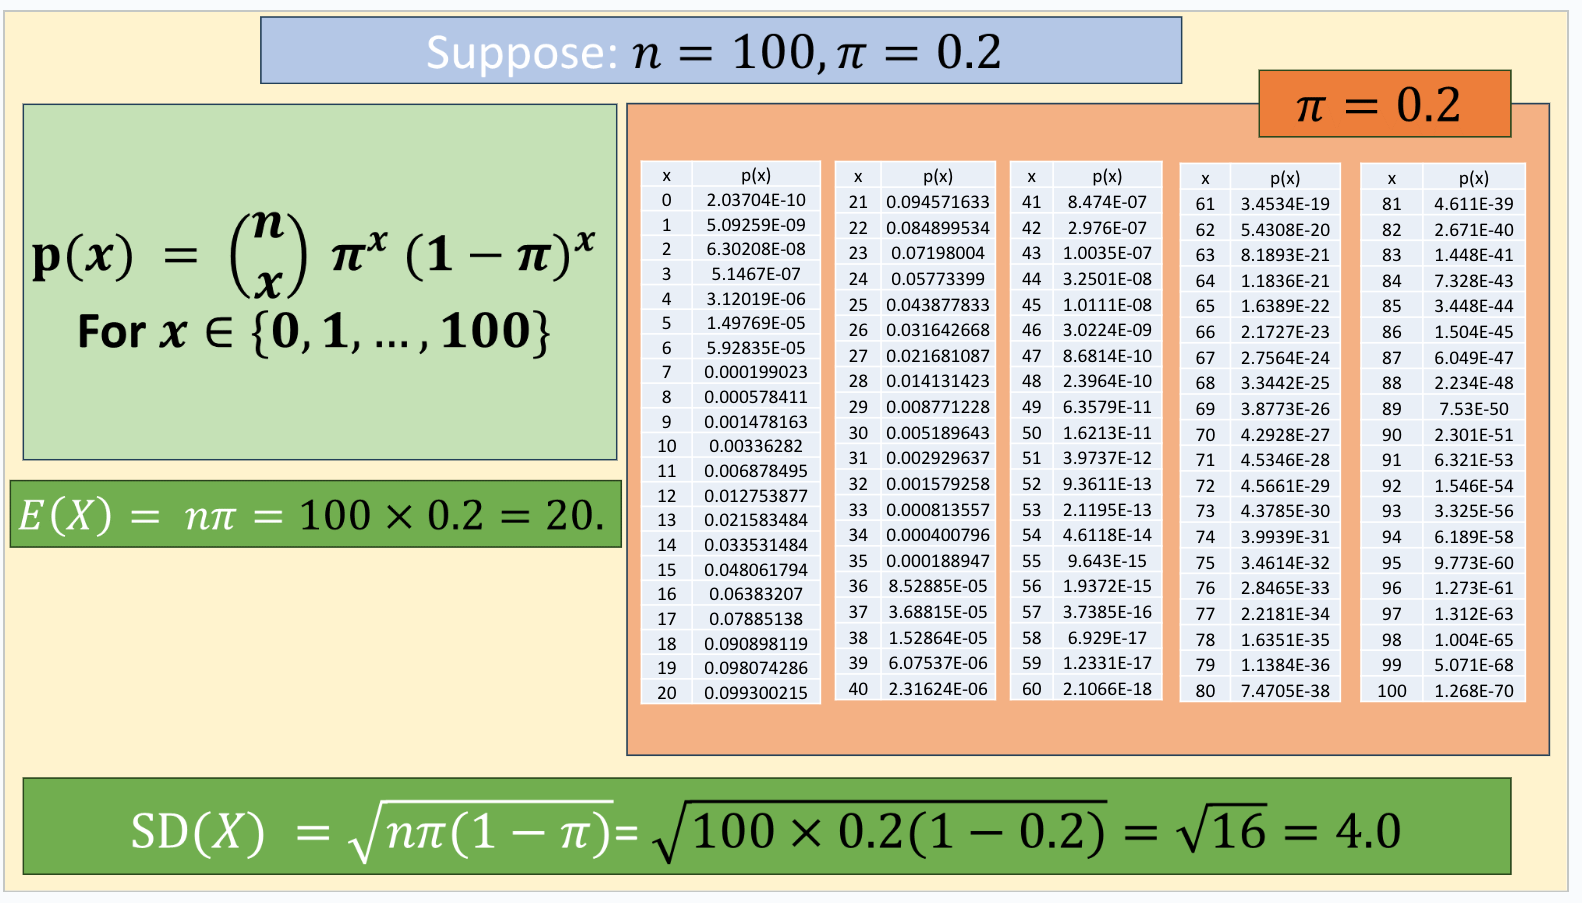
\includegraphics[scale=.45]{figs/BinomialExpectedValue.png}
\end{center}
\vspace{1in}
\end{frame}



\begin{frame}\frametitle{Example}
\vspace{-.1in}
\qbx[4.5in]{amber!50}{
\Exmpl{amber}{} Five fair coins are  flipped.  If the outcomes are assumed independent.
\begin{enumerate}
\item Find the probability mass function of the number of heads obtained.
\item Find the probability that at least 3 heads are obtained.
\item Find the probability that at most 2 heads are obtained.
\end{enumerate}
}\\
\pause
\vspace{.1in}
{\tiny 
{\bf Solution: }
Let $X$ = The number of heads in 5 tossed coins. $X\sim Binomial(n=5, \binP=0.5)$.
\begin{enumerate}
\item $P(X = 0) =0.5^5 = 0.0313$
\item $P(X = 1) ={5 \choose 1}0.5^5 =0.1563$
\item $P(X = 2) ={5 \choose 2}0.5^5 =0.3125$
\item $P(X = 3) ={5 \choose 3}0.5^5 =0.3125$
\item $P(X = 4) ={5 \choose 4}0.5^5 =0.1563$
\item $P(X = 0) ={5 \choose 5}0.5^5 = 0.0313$
\end{enumerate}
}
\end{frame}


\begin{frame}\frametitle{Example}
\vspace{-.1in}
\qbx[4.5in]{amethyst!50}{
\Exmpl{amethyst}{} It is known that screws produced by a certain company will be defective with probability .01, independently of each other. The company sells the screws in packages of 10 and offers a money-back guarantee that at most 1 of the 10 screws is defective. What proportion of packages sold must the company replace? Use the
Binomial Calculator or Statistical Tables.
}\\
\vspace{1.5in}

\end{frame}


\begin{frame}\frametitle{Example}
\vspace{-.1in}
\qbx[4.5in]{olive!50}{
\Exmpl{olive}{} The following gambling game, known as the wheel of fortune (or chuck-a-luck), is quite popular at many carnivals and gambling casinos: A player bets on one of the numbers 1 through 6. Three dice are then rolled, and if the number bet by the player appears i times, i = 1; 2; 3, then the player wins i units; if the number bet by the
player does not appear on any of the dice, then the player loses 1 unit. Is this game fair to the player?
}\\
\vspace{1.5in}
\end{frame}



\setbeamercolor{structure}{fg=airforceblue!70, bg= black!60}



\section{Poisson Distribution  }


\TransitionFrame[airforceblue]{\Large Poisson Distribution  }

\begin{frame}
\begin{itemize}
\qBrd[4.2in]{amber(sae/ece)!40}{
\item[\sqBullet{amber(sae/ece)}] Number of calls received by a customer desk in an hour.
}
\vspace{.1in}\\
\qBrd[4.2in]{atomictangerine!60}{
\item[\sqBullet{atomictangerine}]Number of imperfections in every square-meter of a glass panel used for making LCD TV.
}
\vspace{.1in}\\
\qBrd[4.2in]{bazaar!60}{
\item[\sqBullet{bazaar}] Number of robot malfunctions per day in an assembly line.
}
\vspace{.1in}\\
\qBrd[4.2in]{blush!60}{
\item[\sqBullet{blush}]  Number of car accidents occurs during a year. 
}
\end{itemize}	

\end{frame}


\begin{frame}\frametitle{Poisson Distribution}
The Poisson distribution models the number of occurrences of an
event when there is a known average rate per unit time or space $\lambda$.

\define{Poisson Distribution}{
The requirements for a Poisson distribution are that:
\begin{enumerate}
\item no two events can occur simultaneously,
\item events occur independently in different intervals, and
\item the expected number of events in each time interval remain constant.
\end{enumerate}
}
\end{frame}


\begin{frame}\frametitle{Poisson Distribution: pmf, Expected Value }
The Poisson distribution models the number of occurrences of an
event when there is a known average rate per unit time or space $\lambda$.

\define{Poisson Distribution}{
 A discrete random variable on the support, $\support= \{0,1,2,3, \ldots\}$,  is called a {\bf  Poisson distribution with mean parameter $\lambda$} if the corresponding probability mass function is specified as \\
 $$
\qBrd[1.3in]{amethyst!30}{$ \displaystyle p(x) = \frac{e^{-\lambda}\lambda^x}{x!}$}  $$ { for } $x = 0, 1, 2, 3, \ldots$,  where  $\lambda>0$. 
}
\end{frame}


\begin{frame}
\qBrd[4.6in]{ceil!50}{
\begin{center}
Let $X\sim \text{Poisson}(\lambda)$ 
\end{center}
}\\
\vspace{.5in}
%\qBrd[4.6in]{babyblue!40}{
$\Row{\qBrd[.9in]{airforceblue!50}{\text{Mean}\\
\HLTW{E(X)= \lambda} },  \qBrd[1.5in]{airforceblue!50}{\text{Variance}\\\HLTW{\text{VAR}(X)=  \lambda}}  , \qBrd[1.7in]{airforceblue!50}{\text{MGF}\\\HLTW{\text{M}_{_X}(t)=e^{ \lambda e^t-  \lambda}    }} } $
%}

\vspace{.1in}
\qBrd[4.6in]{airforceblue!50}{
\begin{center}
\qBrd[4.2in]{white!40}{
{
\small
\begin{tabular}{|c|c|c|c|c|c|}
\hline
 Distribution & Support  &  pmf    & Mean   &  Variance  & mgf   \\
& $\support[X]$  &   $\pmf_{_X}(x)$   &  $E(X)$  &   $\text{Var}(X)$  &  $M_{_X}(t)$  \\
 \hline \hline
 & & & & & \\
Poisson$( \lambda)$ &$ \{0, 1, 2, \ldots \}$ & $  \frac{e^{-\lambda}\lambda^x}{x!} $ & $ \lambda$  & $ \lambda$&   $e^{ \lambda e^t-  \lambda}  $   \\
 & & & & & \\
 \hline
  \hline
\end{tabular}
}}\end{center}}
\end{frame}



\begin{frame}
\vspace{1in}
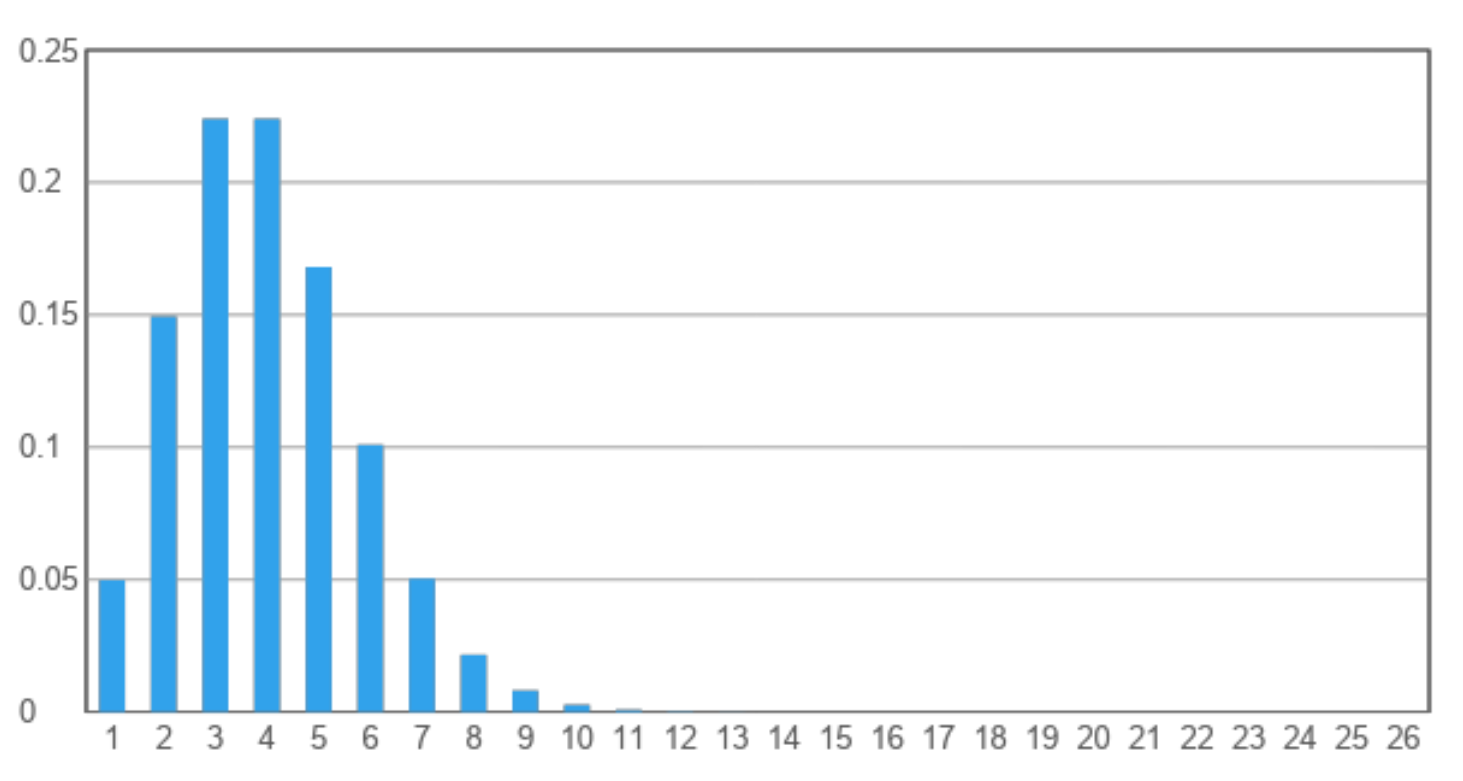
\includegraphics[scale=.3]{figs/PoissonExample1.png}
\end{frame}

{
\setbeamercolor{structure}{fg=brightlavender!80, bg= black!60}


\begin{frame}\frametitle{Reminder from Unit1: Exponential Series $e^x \text{ or }( \exp(x))$}
\vspace{-.1in}
\define{Exponential Series}{
For any real number $x\in \R$, the exponential series $\HLTY{e^x}$  (or sometimes denoted as $\HLTY{\exp(x)}$) is defined as, 
$$\HLTY{\displaystyle e^{x}}=\HLTW{\displaystyle \sum_{n=0}^{\infty}\frac{x^n}{n!}} = \HLTY{\displaystyle 1+\frac{x}{1!}+\frac{x^2}{2!}+ \frac{x^3}{3!}+\cdots,}  $$
}

\vspace{2.5in}


\end{frame}



}


\begin{frame}{Expected Value of Binomial Distribution}
\begin{eqnarray}
M_X(t)& := &  \sum_{y\in \support[X]} e^{ty}\; \pmf_{_X}(y) \nonumber\\
& = &  \sum_{y=0}^{\infty} e^{ty} \frac{e^{-\lambda} \lambda^y}{y!} \nonumber\\
& = &  e^{-\lambda}\sum_{y=0}^{\infty}  \frac{ \left( \lambda e^t\right)^y}{y!} \nonumber\\
& = &  e^{\lambda e^t-\lambda}
\end{eqnarray}



\end{frame}


\begin{frame}\frametitle{ }
\vspace{-.1in}
\begin{enumerate}
\qBrd[4.2in]{chestnut!50}{
\item[\sqBullet{chestnut}]  The number of customers arriving at a service counter within one-hour period.
}\\
\vspace{.1in}
\qBrd[4.2in]{carnationpink!40}{
\item[\sqBullet{carnationpink}] The number of typographical errors in a book counted per page.
}\\
\vspace{.1in}
\qBrd[4.2in]{antiquefuchsia!40}{
\item[\sqBullet{antiquefuchsia}] The number of email messages received at the technical support center daily.
}\\
\vspace{.1in}
\qBrd[4.2in]{chocolate(web)!40}{
\item[\sqBullet{chocolate(web)}] The number of traffic accidents that occur on a specific road  during a month.
}\\
\end{enumerate}
\vspace{.2in}

\end{frame}


\begin{frame}\frametitle{Poisson Process: Most Simple Version
}

\begin{enumerate}
\item The Number of Events Between the interval (can be time-interval or space-interval )  $(s, t]$ follows $$ \text{Poisson}(\lambda\times (t-s))$$
where $\lambda>0$ denotes of rate of events per unit length of the interval. 
\item Events pertaiing to the two distinct intervals are Statistically Independent
\item Rate of occurance of the events remain same for each of the subintervals with same length. 
\end{enumerate}

\end{frame}


\begin{frame}\frametitle{A Few Examples of Poisson Distribution }
\vspace{-.1in}
\qbx[4.5in]{olive!50}{
\Exmpl{olive}{} Messages arrive at an electronic message center at random times, with an average of 9 messages per hour. 
\begin{enumerate}
\item What is the probability of receiving exactly five messages during the next hour?
\item What is the probability that more than 10 messages will be received within the next two hours?
\end{enumerate}
}\\


\vspace{.5in}
{\tiny 
\begin{enumerate}
\item The number of messages received in an hour, $X$ is modeled by
Poisson distribution with $\lambda =  9$, i.e.  $X\sim \text{Poisson}(9)$.
$P(X=5)= \frac{9^5 \exp(-9)}{5!}$
\item The number of messages received within a 2-hour period, $Y$ is
another Poisson distribution with  $Y= (2)(9) =18$, i.e. $Y\sim  \text{Poisson}(18)$.
$P(Y > 10) =1- P(Y\leq 10 )= ...= 0.9696$
\end{enumerate}

}

\end{frame}



%
%\begin{frame}\frametitle{Group Work }
%\begin{enumerate}
%\item Develop a real life example in which you can easily apply:
%\begin{enumerate}
%\item  Group 1: Poisson distribution.
%\item  Group 2: Binomial distribution.
%\item Group 3: Poisson distribution
%\end{enumerate}
%\item  In each case, propose two problems which can be solved using the Statistical Calculator.
%\item Can you propose an idea in which you can mix both distributions?
%(extra)
%\end{enumerate}
%
%\end{frame}




\setbeamercolor{structure}{fg=cambridgeblue!90, bg= black!60}
\section{Geometric Distribution   }
\TransitionFrame[cambridgeblue]{\Large Geometric Distribution}



\begin{frame}\frametitle{Geometric Distribution}
\vspace{-.1in}
\begin{enumerate}
\item Suppose that independent trials, each having a probability $\binP$,
$0 < \binP <1$, of being a success, are performed until a success occurs.
\item Example: The first head in tossing coin several times.
\item Then, Geometric distribution models the number of trials performed until a success occurs.
\end{enumerate}

\define{Geometric Distribution}{
A discrete random variable on the support $\support=\{1,2,3, \ldots \}$ is defined to be the {\bf Geometric($\binP$)}  random variable if the corresponding probability mass function can be represented as the following 
$$\HLTW{\displaystyle p(x) =\binP (1-\binP)^{x-1} }\text{ for } x = 1, 2, 3, \ldots, $$
where $0<\binP<1$.
}

%\qBrd[4.7in]{olive!40}{
%\sqBullet{olive} If $X\sim \text{Geometric}(\binP)$ then $E(X)= \frac{1}{\binP}$, and $\text{Var}(X)= \frac{1-\binP}{\binP^2}$
%}


\end{frame}



\begin{frame}

\qBrd[4.7in]{olive!40}{
\begin{center}
Let $X\sim \text{Geometric}(\binP)$ 
\end{center}
}\\

\vspace{.5in}
%\qBrd[4.6in]{babyblue!40}{
$\Row{\qBrd[.9in]{asparagus!50}{\text{Mean}\\
\HLTW{E(X)= \frac{1}{\binP} } },  \qBrd[1.5in]{asparagus!50}{\text{Variance}\\\HLTW{\text{VAR}(X)=   \frac{1- \binP}{\binP^2}}}  , \qBrd[1.7in]{asparagus!50}{\text{MGF}\\\HLTW{\text{M}_{_X}(t)= \frac{\binP e^t}{1-(1-\binP)e^{t}}    }} } $
%}

\vspace{.1in}
\qBrd[4.6in]{asparagus!50}{
\begin{center}
\qBrd[4.2in]{white!40}{
{
\tiny
\begin{tabular}{|c|c|c|c|c|c|}
\hline
 Distribution & Support  &  pmf    & Mean   &  Variance  & mgf   \\
& $\support[X]$  &   $\pmf_{_X}(x)$   &  $E(X)$  &   $\text{Var}(X)$  &  $M_{_X}(t)$  \\
 \hline \hline
 & & & & & \\
Geometric$( \binP)$ &$ \{1, 2, \ldots \}$ & $\binP (1-\binP)^{x-1}  $ & $ \frac{1}{\binP} $  & $ \frac{1-\binP}{\binP^2} $&   $ \frac{ {\binP} e^t}{1-(1-\binP) e^{t}}    $   \\
 & & & & & \\
 \hline
  \hline
\end{tabular}
}}\end{center}}
\end{frame}


{
\setbeamercolor{structure}{fg=brightlavender!80, bg= black!60}

\begin{frame}\frametitle{Reminder from Unit1: Geometric Series}
\qBrd[4.5in]{babyblue!50}{
Let $p\in \R$ be such that $\abs{p}<1$,  then   $$ \HLTY{\displaystyle \sum_{i=0}^{\infty}p^{i}}= \HLTW{\displaystyle 1+p+p^2+p^3+  \cdots}   =\HLTY{\displaystyle \frac{1}{1-p}}.$$ 
}
\begin{enumerate}
\vspace{.1in}
\item What is the value of $\HLTY{1+0.7+(0.7)^2 + (0.7)^3+ \cdots =}$\\
\vspace{.1in}
\item What is the value of $\HLTY{1-0.7+(0.7)^2 - (0.7)^3+ \cdots =}$
\end{enumerate}
\vspace{3in}
\end{frame}

}




\begin{frame}{Expected Value of Geometric Distribution}
\begin{eqnarray}
M_X(t)& := &  \sum_{y\in \support[X]} e^{ty}\; \pmf_{_X}(y) \nonumber\\
& = &  \sum_{y=1}^{\infty } e^{ty}  (1-\binP)^{y-1}\binP \nonumber\\
& = & \binP   \sum_{z=0}^{\infty } e^{tz+t}  (1-\binP)^{z} \nonumber\\
& = &  \binP e^t   \sum_{z=0}^{\infty } \left((1-\binP)e^{t}\right)^z\nonumber\\
& = & \frac{\binP e^t}{1-(1-\binP)e^{t}} 
\end{eqnarray}



\end{frame}



\begin{frame}\frametitle{Geometric Distribution: Example}
\vspace{-.1in}
\qbx[4.5in]{olive!50}{
\Exmpl{olive}{}  Suppose that the probability of engine malfunction during any one-hour period is $\binP = 0.02$. Find the probability that a given engine will survive two hours.
}\\
\pause

\vspace{.1in}
{\tiny Solution: \\
Letting $Y$ denote the number of one-hour intervals until the first
malfunction, we have 
\begin{eqnarray}
& & P(\text{Survival for Next Two Hours})\nonumber\\
& =&  P(Y\geq 3)\nonumber\\
& =& 1- P(Y\leq 2)\nonumber\\
& = &1-   \sum_{y=1}^{2}p(y)\nonumber\\
& = &1-   \left\{ p(1)+p(2)\right\}\nonumber\\
& =& 1-0.02-0.98\times 0.02\nonumber\\
& =& 0.9604\nonumber
\end{eqnarray}
}
\qBrd[4.5in]{babyblue!70}{
\HLTW{\text{Exercise}}
 Find the mean and standard deviation of Y.
}

\end{frame}



\setbeamercolor{structure}{fg=cadmiumorange!80, bg= black!60}
\section{Negative Binomial Distribution }
\TransitionFrame[cadmiumorange]{\Large Negative Binomial Distribution  }


\begin{frame}
\begin{enumerate}
\item Suppose that independent trials, each having probability  $\binP$,
$0 < \binP < 1$, of being a success are performed until a total of r
successes is accumulated.
\item  Example: The third head in tossing coin several times.

\item  Then, Negative Binomial distribution models the number of trials
performed until a the rth success occurs.
\end{enumerate}

\define{Negative Binomial Distribution}{
Let $\binP \in (0,1)$ and $r$ be a positive integer. 
A discrete random variable on the support $\support=\{r+1,r+2,r+3, \ldots \}$ is defined to be the {\bf Negative-Binomial($r, \binP$)}  random variable if the corresponding probability mass function can be represented as 
$$\HLTW{ \displaystyle p(x) ={{x-1}\choose{r-1}}\binP^{r} (1-\binP)^{x-r} }\text{ for } x = r+1, r+2,r+ 3, \ldots, $$
}

%\qBrd[4.7in]{olive!40}{
%\sqBullet{olive} If $X\sim \text{Negative-Binomial}(r, \binP)$ then $E(X)= \frac{r}{\binP}$, and $\text{Var}(X)= \frac{r(1-\binP)}{\binP^2}$
%}


\end{frame}






\begin{frame}
\qBrd[4.7in]{amber!40}{
\begin{center}
Let $X\sim \text{Negative-Binomial}(r, \binP)$
\end{center}
}\\

\vspace{.5in}
%\qBrd[4.6in]{babyblue!40}{
$\Row{\qBrd[.9in]{carrotorange!50}{\text{Mean}\\
\HLTW{E(X)= \frac{r}{\binP} } },  \qBrd[1.5in]{carrotorange!50}{\text{Variance}\\\HLTW{\text{VAR}(X)=   \frac{r(1- \binP)}{\binP^2}}}  , \qBrd[1.7in]{carrotorange!50}{\text{MGF}\\\HLTW{\text{M}_{_X}(t)=\left( \frac{\binP e^t}{1-(1-\binP)e^{t}}\right)^r    } } } $
%}

\vspace{.1in}
\qBrd[4.75in]{carrotorange!70}{
\begin{center}
\qBrd[4.7in]{white!40}{
{
\tiny
\begin{tabular}{|c|c|c|c|c|c|}
\hline
 Distribution & Support  &  pmf    & Mean   &  Variance  & mgf   \\
& $\support[X]$  &   $\pmf_{_X}(x)$   &  $E(X)$  &   $\text{Var}(X)$  &  $M_{_X}(t)$  \\
 \hline \hline
 & & & & & \\
Negative-Binomial$(r,  \binP)$ &$ \{r+1, r+2, \ldots \}$ & $ {{x-1}\choose{r-1}}\binP^{r}(1-\binP)^{x-r}  $ & $ \frac{r}{\binP} $  & $ \frac{r(1-\binP)}{\binP^2} $&   $\left( \frac{  \binP e^t}{1-(1-\binP) e^{t}}  \right)^r  $   \\
 & & & & & \\
 \hline
  \hline
\end{tabular}
}}\end{center}}
\end{frame}





\begin{frame}\frametitle{Geometric Distribution: Example}
\vspace{-.1in}
\qbx[4.5in]{amber!50}{
\Exmpl{amber}{}{
A machine produces 1\% defective parts. Using the statistical calculator, calculate the probability that
\begin{enumerate}
\item 10 parts have to be selected until to get 2 defective parts.
\item Between 20 to 25 parts have to be selected to get 2 defective parts.
\end{enumerate}
}  
}\\
\pause

\vspace{1in}
{\tiny Solution: \\

}
\qBrd[4.5in]{babyblue!70}{
\HLTW{\text{Exercise}}
 Find the mean and standard deviation of Y.
}

\end{frame}



\setbeamercolor{structure}{fg=antiquefuchsia!80, bg= black!60}
\section{Miscellaneous Problems}

\TransitionFrame[antiquefuchsia]{\Large Miscellaneous Problems  }



\begin{frame}\frametitle{}
\vspace{-.1in}
\qbx[4.5in]{olive!30}{
\Exmpl{olive}{}{
Approximately 10\% of the glass bottles coming off a production line have serious flaws in the glass. If two bottles are randomly selected, find the mean and variance of the number of bottles
that have serious flaws.
}  
}\\
\vspace{2.5in}

\end{frame}








\begin{frame}\frametitle{}
\vspace{-.1in}
\qbx[4.5in]{airforceblue!30}{
\Exmpl{airforceblue}{}{
Cars arrive at a toll both according to a Poisson process with mean 80 cars per hour. If the
attendant makes a one-minute phone call, what is the probability that at least 1 car arrives
during the call?
}  
}\\
\vspace{2.4in}
\end{frame}








\begin{frame}\frametitle{}
\vspace{-.1in}
\qbx[4.5in]{teal!30}{
\Exmpl{teal}{}{
Suppose that a lot of  electrical fuses contains 5\% defectives. If a sample of 5 fuses is tested, find the probability of observing at least one defective.
}  
}\\
\vspace{2.6in}
\end{frame}




\begin{frame}\frametitle{}
\vspace{-.1in}
\qbx[4.5in]{amber!30}{
\Exmpl{amber}{}{
An oil exploration firm is formed with enough capital to finance ten explorations. The probability of a particular exploration being successful is 0.10  . Assume the explorations are independent.
\vspace{-.1in}
\begin{enumerate}
\item Find the mean and variance of the number of successful explorations.
\item Suppose the firm has a fixed cost of \$20,000 in preparing equipment prior
to doing its first exploration. If each successful exploration costs \$30,000 and each unsuccessful
exploration costs \$15,000, find the expected total cost to the firm for its ten explorations.
\end{enumerate}
}  
}\\

\vspace{2in}
\end{frame}


\begin{frame}\frametitle{}
\vspace{-.1in}
\qbx[4.5in]{blue!25}{
\Exmpl{blue!50}{}{
A food manufacturer uses an extruder (a machine that produces bite-size cookies and snack food) that yields revenue for the firm at a rate of \$200 per hour when in operation.  However, the
extruder breaks down an average of two times every day it operates. If Y denotes the number of breakdowns per day, the daily revenue generated by the machine is $\HLTW{R=1600-50Y^2}$. Find the expected daily revenue for the extruder.
}  
}\\

\vspace{2in}
\end{frame}



\begin{frame}\frametitle{}
\vspace{-.1in}
\qbx[4.5in]{babyblue!30}{
\Exmpl{babyblue!80}{}{ A particular sale involves four items randomly selected from a large lot that is known to contain 10\% defectives.  Let Y denote the number of defectives among the 20 sold. The purchaser of the items will return the defectives for repair, and the repair cost is given by $\HLTW{\text{Cost} = 3Y^2 + Y + 2}$.  Find the expected repair cost.
}  
}\\

\vspace{2in}
\end{frame}



\begin{frame}\frametitle{}
\vspace{-.1in}
\qbx[4.5in]{apricot!40}{
\Exmpl{apricot!80}{}{ In a certain population,  it is known that 80\% of the individuals have the Rhesus (Rh) factor present in their blood.   
\begin{enumerate}
\item If 5 volunteers are randomly selected from the population, what is the probability that at least one does not have the Rh factor?
\item If five volunteers are randomly selected, what is the probability that at most four have the Rh factor?
\end{enumerate}
}  
}\\

\vspace{2in}
\end{frame}



\begin{frame}\frametitle{}
\vspace{-.1in}
\qbx[4.5in]{amethyst!30}{
\Exmpl{amethyst!80}{}{ \small Consider rolling a fair dice multiple times untill the first 6 appears.  
\begin{enumerate}
\item Find the expected number of throws required to get the first 6.
\item What is the probability that more then 8 throws are required to obtain the first 6? 
\end{enumerate}
}  
}\\

\vspace{2in}
\end{frame}






\begin{frame}\frametitle{}
\vspace{-.1in}
\qbx[4.5in]{asparagus!30}{
\Exmpl{asparagus!80}{}{ \small A tollbooth operator has observed that cars arrive randomly at a rate of 360 cars per hour
\begin{enumerate}
\item what is the probability that exactly two cars will come during a specific one-minute period?
\item Find the probability that 40 cars arrive between 10 am to 10:10 am 
\item Find the expected number of cars between 10 am to 10:10 am
\end{enumerate}
}  
}\\

\vspace{2in}
\end{frame}






\TransitionFrame[antiquefuchsia]{\Large Questions?  }
 
 
\end{document}
